\documentclass{article}
\usepackage{graphicx}
\usepackage{wrapfig}
\usepackage{filecontents}
\usepackage{siunitx}
\usepackage[table]{xcolor}
\usepackage{float}
\usepackage{hyperref}

\usepackage{color} % balíček pro obarvování textů
\usepackage{xcolor}  % zapne možnost používání barev, mj. pro \definecolor
\usepackage[total={175mm,230mm}, top=23mm, left=20mm, includefoot]{geometry}
\hypersetup{
    colorlinks,
    linkcolor={blue!50!black},
    citecolor={green!50!black},
    urlcolor={blue!80!black}
}
\definecolor{orange}{RGB}{ 251, 114, 032}
\definecolor{fialova}{RGB}{ 255, 000, 255}

\newcommand \obr[1]
{ obr. \ref{#1}}

\newcommand \tab[1]
{ tab. \ref{#1}}


% \usepackage{lmodern}
% \usepackage{amssymb,amsmath}
% \usepackage{ifxetex,ifluatex}
% \usepackage{fixltx2e} % provides \textsubscript
% \ifnum 0\ifxetex 1\fi\ifluatex 1\fi=0 % if pdftex
%   \usepackage[T1]{fontenc}
%   \usepackage[utf8]{inputenc}
% \else % if luatex or xelatex
%   \ifxetex
%     \usepackage{mathspec}
%   \else
%     \usepackage{fontspec}
%   \fi
%   \defaultfontfeatures{Ligatures=TeX,Scale=MatchLowercase}
% \fi

% \usepackage{pgfplots} % http://www.chiark.greenend.org.uk/doc/texlive-doc/latex/pgfplots/pgfplots.pdf
% \usepackage{blindtext}

% \usepackage{subfiles} % Best loaded last in the preamble

% \usepackage{bookmark}
% \usepackage{tikz}
% \usetikzlibrary{patterns}

% \usepgfplotslibrary{polar}
% \usepgfplotslibrary{external}
% \usepgfplotslibrary{fillbetween}

\begin{document}
\section{Pracovní bod a jeho pohyb}

Tranzistor je typická nelineární součástka v obvodu popsatelná šesti veličinami, třemi proudy a třemi napětími vyznačenými na \obr{pracovni_bod_tranzistoru} a) (\(I_C I_B I_E U_{CE} U_{BE} U_{BC})\).
Tyto veličiny jsou propojeny nelineárními závislostmi které lze chápat jako šestirozměrný objekt, kterým když provede dvourozměrný řez dostaneme např. výstupní charakteristiku (závislost \(I_C\) na \(U_{CE}\)
při konstantním proudu \(I_B\)).
\vspace{-1mm}
\begin{figure}[H]
    % \centering
    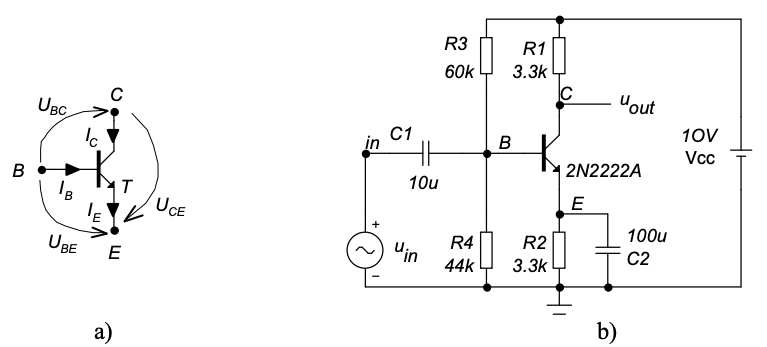
\includegraphics[width=\textwidth]{pracovni_bod_tranzistoru.png}
    \caption{\label{pracovni_bod_tranzistoru}}
\end{figure}

Pokud tranzistory zapojíme do zapojení na \obr{pracovni_bod_tranzistoru} b) při \(U_{in} = 0\) ustálí se jeho veličiny na konkrétním bodě, tento bod označujeme \(Q\) a nazýváme ho stejnosměrný pracovní bod tranzistoru.
Aby mohl tranzistor fungovat jako zesilovač správně je nutné aby nastavení pracovního bodu umožňovalo v oběma směry dostatečný rozkmit výstupního signálu v dostatečné míře bez přílišného zkreslení.
Pracovní bod se proto obvykle nastavuje tak aby v ustáleném stavu platilo \(U_{out} = \frac{1}{2}V_{cc}\)

\vspace{1mm}
\begin{wrapfigure}{r}{0.5\textwidth}
  % \centering
  \vspace{-10mm}
  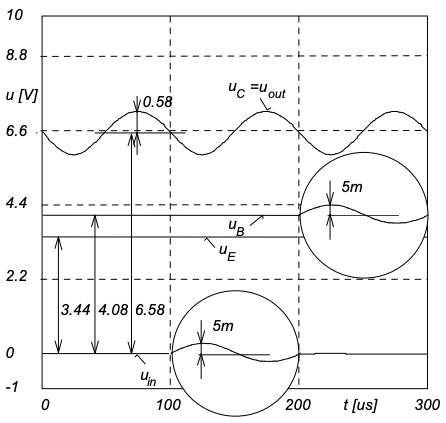
\includegraphics[width=0.5\textwidth]{vstup-baze-vystup.png}
  \caption{\label{vstup_baze_vystup}}
\end{wrapfigure}
Abychom mohli na tento zesilovač přivést signál s jiným středním napětím neš jaké je na bázi tranzistoru, přípojíme vstup zesilovače na bázi skrz kapacitu \(C_1\).
Tato kapacita musí být dostatečně velká aby se pro signál o požadované frekvenci dala považovat za zkrat.
Na \obr{vstup_baze_vystup} je zobrazen možný procházející signál.

Při nastavování pracovního bodu je mimo jiné nezbytné znát následující vztahy
\begin{equation}
    I_C=I_B\cdot\beta \quad \quad I_{E}=I_{B}+I_{C}
    \label{proud_kolektoru}
\end{equation}
\newpage

\section{Počítačové cvičení}
\begin{figure}[H]
  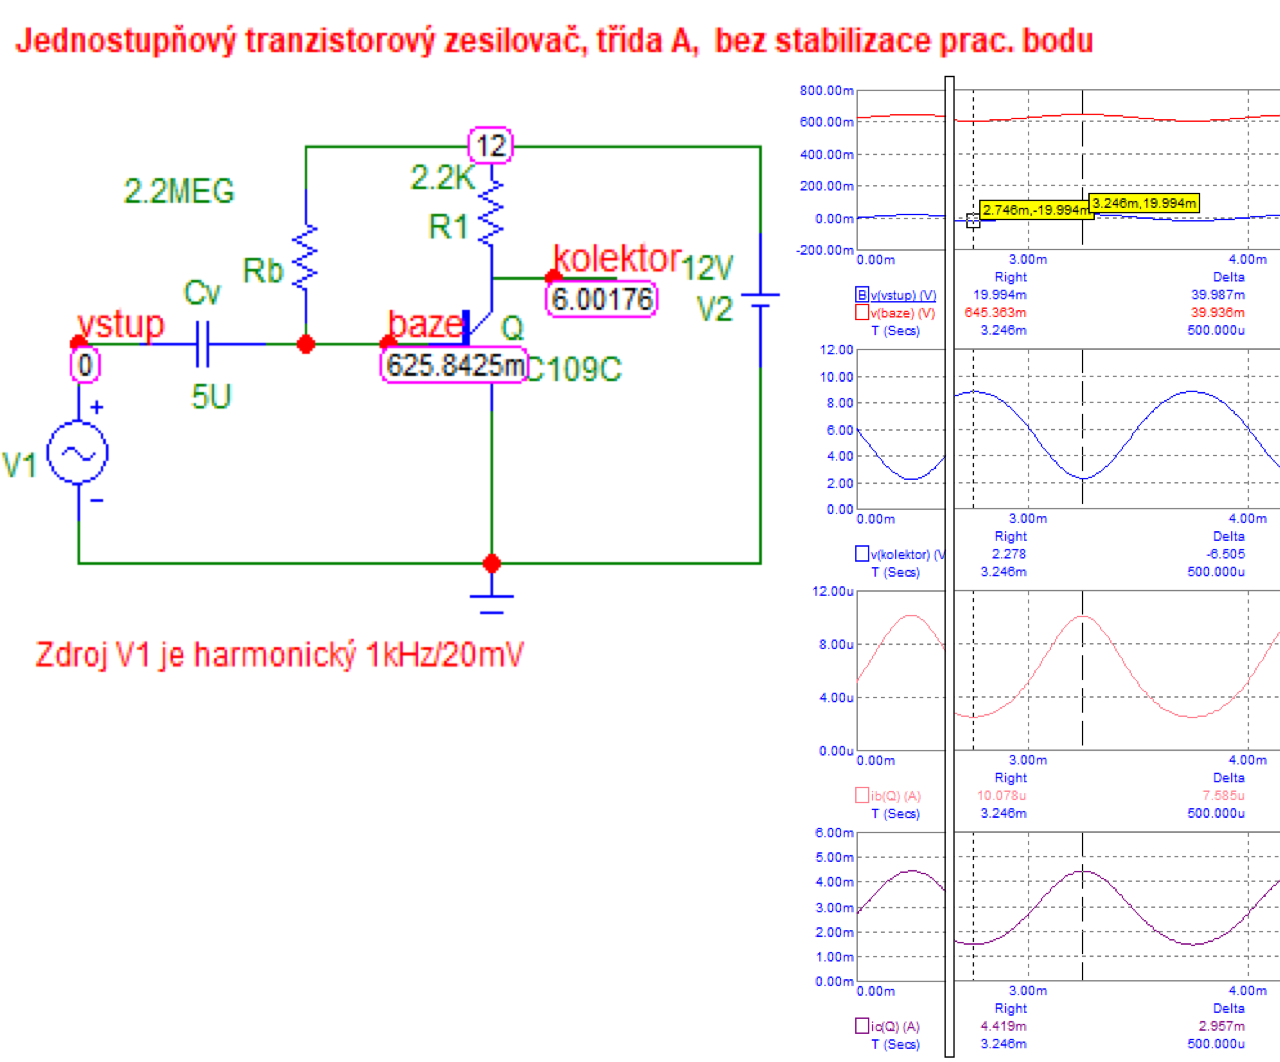
\includegraphics[width=\textwidth]{PC/BJT/prac_bod_sim_1.png}
  % \addlegendentry{test}
  \caption{\label{prac_bod_sim_1} Stejnosměrné nastavení pracovního bodu a~odezva na základní sinusoví signál}
\end{figure}

\begin{figure}[H]
  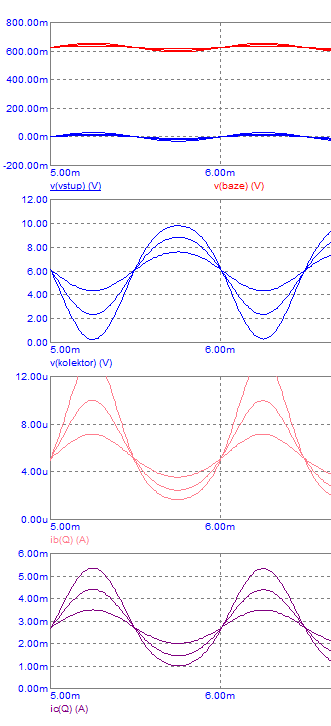
\includegraphics[width=0.3\textwidth]{PC/BJT/Tranzient_analyza_3.png}
  % \addlegendentry{test}
  \caption{\label{prac_bod_sim_1} Sinusový průběh při pohybu pracovního bodu}
\end{figure}


\section{Laboratorní cvičení}
% \subsections{zadání}
% Nejprve sestavte obvod bez vazebního kondenzátoru a zdroje signálu. Změnou odporu Rb
% nastavte ss napětí na kolektoru tranzistoru 6 V. Změřte všechna uzlová napětí a z nich dopočtěte
% větvové proudy. Porovnejte s výsledky z NC a PC.
% Doplňte obvod o Cv a generátor signálu. Proveďte „oživení“ zesilovače pomocí osciloskopu.
% Zesilovač nesmíte přebudit výstupní napětí nesmí vykazovat zkreslení. Měřte při kmitočtu
% 1 kHz. Zakreslete časové průběhy vstupního napětí, napětí na bázi a na kolektoru, včetně ss
% posunutí. Změřte amplitudy a vypočtěte z nich střídavá zesílení.

\begin{wrapfigure}{r}{0.5\textwidth}
  % \centering
  \vspace{-10mm}
  % \hspace{5mm}
  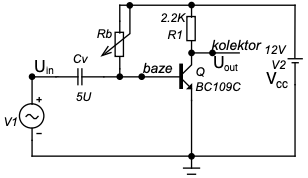
\includegraphics[width=0.5\textwidth]{obvod-z-laborky.png}
  \caption{\label{obvod_z_laborky}}
\end{wrapfigure}
Měřili jsme s tranzistorem BC55 u kterého jsme na začátku naměřili \(\beta = 422\)
Nejprve jsme sestavili obvod a pomocí potenciometru jsme nastavili pracovní bod dle \tab{tab_pracovni_bod}.

\begin{tabular}{|c|c||c|c|}
  \hline
  \(U_{cc}\-[V]\) & \(U_{c}\-[V]\)  & \(R_b\)  &	\(R_c\)   \\ \hline
  12              &                 &          &            \\ \hline

  \label{tab_pracovni_bod}
\end{tabular}

\end{document}
